\section{Interpreter}
For \textit{Times, Divide, And, Or, Not} and \textit{Negate} the general idea is to first evaluate the expressions, and then pattern match the resulting expressions' type. If successful then return the result, otherwise we throw an error. For \textit{And} and \textit{Or} we have nested pattern matching in order to achieve short circuiting. This is all implemented on lines 165 - 207 of Interpreter.fs.\\
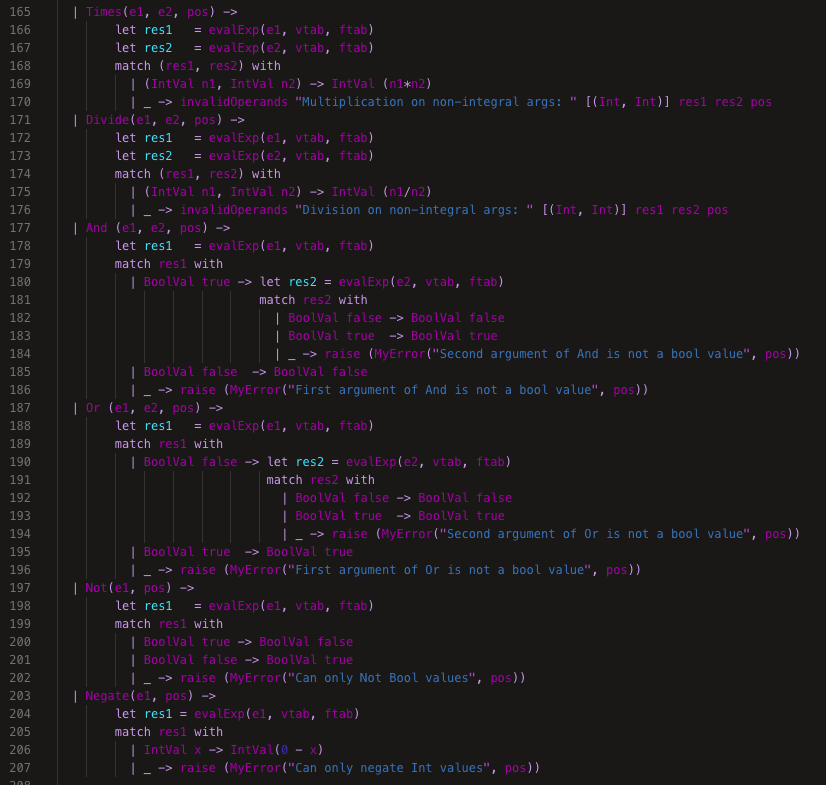
\includegraphics[width=\linewidth]{Materials/Interpreter/Expressions}\\
The functions are implemented somewhat similarly by first evaluating the expressions and then match the resulting expressions' types.\\
Replicate pattern matches for its first argument being of type int and being grater or equal to zero and for the second argument to be of type int, bool or char. If it succeeds it uses the f\# function 'List.replicate' to construct the output. (lines 300 - 308).\\
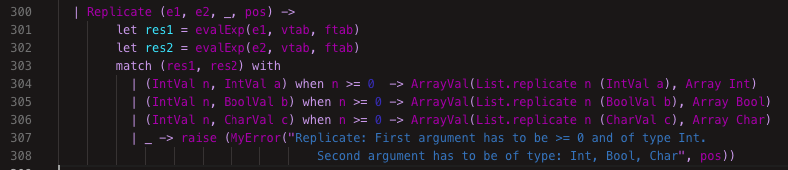
\includegraphics[width=\linewidth]{Materials/Interpreter/Replicate}\\
Filter matches its second argument with an array. If it succeeds it uses the f\# function 'List.filter' to create the output. But to make sure the first argument return bool, a lambda expression is passed to List.filter which pattern matches the output of the function passed to Filter with bool values. (lines 319 - 333).\\
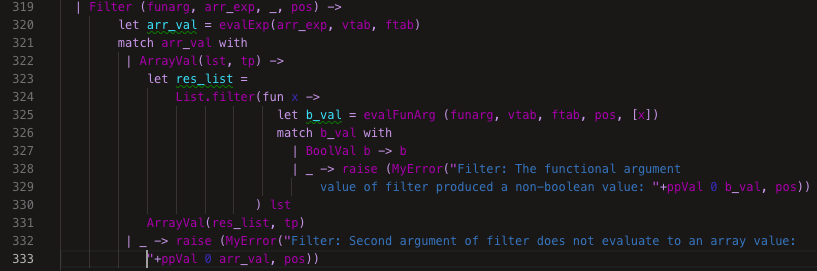
\includegraphics[width=\linewidth]{Materials/Interpreter/Filter}\\
Scan works similarly as the previous functions, as it pattern matches an array and if it succeeds it uses the f\# function 'List.scan' to construct the output. (lines 339 - 347).\\
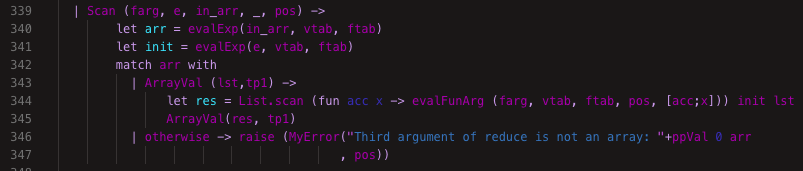
\includegraphics[width=\linewidth]{Materials/Interpreter/Scan}\\